\documentclass{article}\usepackage[]{graphicx}\usepackage[]{color}

\usepackage{alltt}
\usepackage{float}
\usepackage{graphicx}
\usepackage{tabularx}
\usepackage{siunitx}
\usepackage{amssymb} % for math symbols
\usepackage{amsmath} % for aligning equations
\usepackage{textcomp}
\usepackage{booktabs}
\usepackage{mdframed}
\usepackage{natbib}
\usepackage{comment}
\usepackage[colorinlistoftodos]{todonotes} % to make comments on the margin
\usepackage[small]{caption}
\setlength{\captionmargin}{30pt}
\setlength{\abovecaptionskip}{0pt}
\setlength{\belowcaptionskip}{10pt}
\topmargin -1.5cm        
\oddsidemargin -0.04cm   
\evensidemargin -0.04cm
\textwidth 16.59cm
\textheight 21.94cm 
%\pagestyle{empty} %comment if want page numbers
\parskip 7.2pt
\renewcommand{\baselinestretch}{1.5}
\parindent 0pt
%\usepackage{lineno}
%\linenumbers

%% R Script

\title{Unravelling the phenology-phylogeny tangle.}

% alternative titles:
%% An expanded bayesian phylogenetic mixed model to unravel the phenology-phylogeny tangle. %% this sounds too methodsy

\begin{document}

\maketitle

\noindent Authors:\\
The Wolkovich Lab in 2019 \& collaborators $^{1,2,3,4}$ % Will Pearse, Jonathan Davies also
\vspace{2ex}\\
\emph{Author affiliations:}\\
$^{1}$Forest \& Conservation Sciences, Faculty of Forestry, University of British Columbia, 2424 Main Mall, Vancouver, BC V6T 1Z4;\\
$^{2}$Arnold Arboretum of Harvard University, 1300 Centre Street, Boston, Massachusetts, USA;\\
$^{3}$Organismic \& Evolutionary Biology, Harvard University, 26 Oxford Street, Cambridge, Massachusetts, USA;\\
$^{4}$Edificio Ciencias, Campus Universitario 28805 Alcalá de Henares, Madrid, Spain\\
 

\vspace{2ex}
$^*$Corresponding author: ignacio.moralesc@uah.es\\
\renewcommand{\thetable}{\arabic{table}}
\renewcommand{\thefigure}{\arabic{figure}}
\renewcommand{\labelitemi}{$-$}
\setkeys{Gin}{width=0.8\textwidth}

%%%%%%%%%%%%%%%%%%%%%%%%%%%%%%%%%%%%%%%%%%%%%%%
%%%%%%%%%%%%%%%%%%%%%%%%%%%%%%%%%%%%%%%%%%%%%%%
\clearpage

\begin{comment}
\section*{Rationale \& Significance}

Previous work has looked at the phylogenetic conservatism of phenology across plant species, finding that, first flowering is significantly conserved \citep{davies2013phylogenetic} and, when using OU models so are shifts in first flowering and the slopes of the relationship between flowering and year \citep{rafferty2017global}. Research in this area has focused on the phenotype (phenological event or its shifts) rather than on the cues---i.e. how shifts in the environment trigger species responses. Beyond whether or not phenology is phylogenetically conserved, determining evolutionary constraints in phenological responses to temperature and daylight, may have deeper implications for forecasting under ongoing change.\\ 

Nevertheless, previous work on the phylogenetic conservatism of phenology has still not addressed:\\

- Emphasis has been put on the phenotype rather than on the cues\\
- Are phenological responses in lab experiments conserved as well? In \cite{joly2019importance} the authors check this with a focus on intraspecific variations\\
- How the sensitivities to different environmental cues are conserved?\\
- Are the responses to certain cues more strongly conserved than to others?\\
- How does accounting for phylogeny affects model estimations of cue sensitivity?\\

And beyond work on phylogenetic conservatisms, previous comparative research on phenological responses to cues (experimental or observational) has either:\\

- Ignored phylogenetic relationships (or the fact that species are not independent units)\\
- Accounted for phylogenetic relationships assuming that they are \emph{stationary} across predictors-traits and can be modelled by including phylogenetic Variance-Covariance in model residuals. This is the rationale behind common-use PGLS approaches but it \"hides\" the partial phylogenetic constraints to model predictors.\\ 

An overlooked question so far is whether we could gain any additional information by accounting for independent phylogenetic structuring in each species responses to each predictor in a multi-linear response model setting. Typical methods are good to account for species non-independence but provide little insight relative to phylogenetic effects on each predictor.
\todo{I think the new approach is a bit of a game changer as it shifts the focus from empirical results of phylo-constrains on phenology to a more methodsy paper. We need to decide a focus.}



The potential interest of findings in this direction stem from:\\
- better predictions of phenology (or need to account for it in models)\\
- better understanding of the mechanistic basis of plant responses to climate\\
- better design the next generation of experiments \\


## bits from previous version of the abstract to remove at a later stage

The plasticity of these responses may ultimately determine species ability to withstand ongoing environmental change because non-plastic species may undergo developmental events under unadequate conditions---e.g. a species advancing flowering too much could see increased the risk of frost events. Phenology describes the responses to seasonal change in environmental cues and while it is often regarded to as a rather plastic trait, it is still unknown whether or not phenology is a phylogenetically conserved trait. 


\end{comment}

\section*{Abstract}

Plants have evolved responses to environmental cues able to inform them about the temporal distribution of key resources---i.e. energy and light. The responses to individual cues such as forcing (or spring warming) have shown to be subjected to some degree of evolutionary conservatism. Yet, plants do not respond to isolated cues but to a combination of interacting cues, which difficults accurate predictions of phenology in the face of environmental change. Whether and how evolution has constrained phenological responses to combinations of interacting cues is not yet understood even when this knowledge could enhance model predictions and inform how different plant lineages have adapted to environmental change along their evolutionary histories. Here we use Bayesian hierarchical models and the most complete dataset on tree species phenological responses measured in experimental conditions to: (a) test if phenological responses to three major interacting cues are conserved phylogenetically when considered jointly, (b) compare the phylogenetic signal in the responses to different cues and, (c) test whether coefficient estimates differ between models assuming phylogenetic independence among species and models that explicitly incorporate phylogeny. Results show non-random phylogenetic structuring of phenological responses, highly variable across species and cues. More interestingly, regression coefficients shift when models control for phylogenetic effects, particularly so for forcing, which becomes the most important cue. Taken together, our results suggest that phylogeny should be incorporated into studies modelling multi-species phenological responses, as such responses have been jointly constrained through evolution and thus are not independent.  


\begin{comment}
\begin{enumerate}
\begin{enumerate}
\item How plants respond to environmental cues--i.e. temperature, daylight--may determine their resilience or vulnerability to ongoing climate change. 
\item Phenology provides a good description of plant responses to to the environment. 
\item Phenology has been regarded to as a rather plastic trait, thus with a lot of variation both intra- and inter-specifically.
\item Variation in phenology could have randomly accummulated across species (and then phenology would be an evolutionary labile trait), or be structured in the phylogeny so that closely related species resemble more each other in their phenological responses (conserved trait).
\item Whether or not phenology is conserved has implications for the need to account for phylogenetic autocorrelation in cross-species analyses.
\item More interestingly, given that phylogeny can act as a proxy for other (unaccounted) traits that may be linked to phenology, including it in models could lead to more accurate predictions.
\item Here we use Bayesian hierarchical models and the most complete dataset on tree species phenological responses measured in experimental conditions to: (a) test if tree species responses to cues are conserved phylogenetically, (b) compare the phylogenetic signal in the responses to different cues and, (c) test the abiltiy of phylogenetically informed models to improve predictive accuracy of phenology.
\item Results show non-random phylogenetic structuring of phenological responses, highly variable across cues.  
\item Taken together, our results suggest that phylogeny should be incorporated into studies modelling multi-species phenological responses, as such responses have been constrained through evolution and thus are not independent.  
\end{enumerate}
\end{comment}

% not yet satisfied about the pitch - this is already said in Davies et al. 2013 
% should we emphasize the fact that we are using experimental/lab data? What are the gains with respect data from the field?

% we need an angle of at least some novelty

%%%%%%%%%%%%%%%%%%%%%%%%%%%%%%%
% Introduction
%%%%%%%%%%%%%%%%%%%%%%%%%%%%%%%
% Meeting call notes: https://github.com/lizzieinvancouver/ospree/wiki/Phylogeny-and-phenology


\section*{Introduction}

\begin{comment}
\begin{enumerate}
\item Predicting species responses to recent anthropogenic climate change presents a major challenge to ecological forecasting
\begin{enumerate}
\item On average global temperatures are warming, but there is regional and seasonal variation behind this average and shifts along other climate axes such as precipitaion are more complex than simple increases % or  but climate change is atcually multivariate and complex
\item Over the past few decades empical studies have suggested that plants are shifting in their geographical distributions, moving to more northern latitudes and elevations, and shifting the timing of their life cycles
\item However, responses are highly variable across species.
\item Understanding how different species lineages have evolved their phenotypic responses to the combined effects of environmental change would greatly aid prediction
\end{enumerate}
\end{comment}
Forecasting remains a major challenge in ecology, especially as anthropogenic climate change drives demand for more accurate forecasts across species. As global temperatures warm, plant species are shifting the timing of their life cycles \citep{Cleland:2007or} and their geographical distributions towards higher latitudes and altitudes \citep{chen2011}, but responses are highly variable across species \citep{menzel2020}. Some of this variability is due to the complexity of climate change itself---the regional and seasonal variation in warming underlying average trends and shifts in other climate axes (e.g. precipitation)---however, much of it is driven by species-specific variation in response to environmental change, which we can only predict for a few well-studied species. More accurate forecasts will require efforts to scale our understanding across more plant species. Understanding how different plant lineages have evolved their phenotypic responses to the combined effects of multiple dimensions of environmental change would greatly aid prediction.\\ %the last sentence feels a bit general still - try better connection with next paragraph

\begin{comment}
\item Environmental cues matter as they inform organisms about the temporal distribution of key resources.
% Understanding how different plant lineages have evolved their phenotypic responses to the joint effects of interacting environmental cues remains a challenge. % Lizzie says: I like this, but the introduce of cues and lineages at once feels too much at the very start... suggested alternative intro, but take or leave what works!
\begin{enumerate}
\item Responses (and their evolution) to cues are usually studied individually assuming that a given phenotypic response (e.g. time of leafout) is linked to a single cue, when likely multiple ones operate interactively (and have done so across evolutionary history) to shape that response. 
\item For example, light, nutrients and water often determine growth rates and size
\item Or how the timing of many recurring life cycle events (phenology) is determined by a combination of temperature and light. 
\end{enumerate}
\end{comment}
Decades of research show that plants use environmental cues to time their phenotypic responses with the temporal distribution of key resources and to avoid periods of high abiotic or biotic stress \citep{larcher1980,Chuine2000}. Commonly, responses to environmental cues, and their evolution, are studied individually, assuming that a given phenotypic response is predominantly linked to a single cue: for example, that time of leafout is driven by summed heat during early spring \citep{Wolkovich:2012n,davies2013phylogenetic}. Such efforts ignore a more likely scenario for most phenotypic traits where multiple cues interacting along evolutionary history have shaped plant responses \citep{}. For example, species-level growth rates or plant height may be determined by the interaction among several cues---e.g. soil nutrients, water availability and light \citep{larcher1980}. Similarly, the timing of recurring life cycle events (phenology) is determined by a combination of temperature and light \citep{chuinearees}.\\

\begin{comment}
\item Phenology makes for an ideal study case of species' responses to interacting environmental cues.
\begin{enumerate}
\item Phenology is a critical trait to studying biological responses to climate change.
\item In temperate species its cue system is generally known: forcing, chiling, photoperiod
\item It is amongst the few phenotypic characters (if any other exists) for which there are multi-species experimental data on its responses to the three major environmental cues. 
\item Out of these three major cues that affect plants, few multi-species analyses have considered all three simultaneously, with repeated consensus that chilling and forcing would prevail, but would this pattern hold if evolution/phylogeny was accounted for? % or perhaps avoid talking about phenology yet and making this opening more general about traits and phenotypes and their response to cues: from Lizzie's notes: the trait is a phenotype itself is made of underlying traits that respond to different cues. (For example, plant height or growth is a function of responses to water and nutrients.)
 \end{enumerate}
% My suggestion is a paragraph on a pheno by phylo, then one one on phylo methods (short), but you could have an additional paragraph on more pheno x phylo, see commented out chunk below
\end{comment}
Phenology may provide an ideal case study to gain insights on how species responses to interacting environmental cues have evolved because the basic cue system is well established \citep{chuinearees}. In temperate plants, phenology is generally determined by forcing---warm temperatures during the growing season, chilling---cool temperatures during dormancy period over winter, and photoperiod \citep{chuinearees}. Further, phenology is one of few phenotypic traits where decades of research provide multi-species experimental data on plant responses to these three major cues. Recent multi-species analyses considering forcing, chilling and photoperiod have shown that chilling and forcing together determine complex non-linear responses to warming \citep{flynn2018,ettinger2020}, complicating forecasting. In addition, studies found remarkable variation across species in their responses to cues, raising the question of whether such variation is phylogenetically structured. If phylogenetically close species have evolved similar responses to cues it could facilitate forecasting to unmeasured species, and provide insights into how cues have evolved in the past. \\

\begin{comment}
\item Phenology x phylogeny quick review ...
\begin{enumerate}
\item It is evolutionary conserved (to some extent, review antecedents).
\item Research in this area has focused on the phenotype (phenological event or its shifts) rather than on the cues---i.e. how shifts in the environment trigger species responses. For example, first flowering is significantly conserved \citep{davies2013phylogenetic}. 
\item Whether shifts in first flowering over time are also conserved is less clear and all inference to date is based on observational data, where geographical signals in phylogeny may drive trends attributed to phenology \citep[e.g.,][]{rafferty2017global}, as discussed in \citep{davies2013phylogenetic}. % This Rafferty paper is so flawed analytically that I suggest we better couch how we cite it ... see what you think... could also check Pearse NEE paper for how phylogeny affected answers
\item Further, additional questions remain open: in a multi-species context, have specific lineages adapted more strongly to some of the cues? or to any combination of cues? Is there any cue that is particularly labile?
\item Answering these questions may: (i) inform about the need to account for phylogeny in phenological models and predictions, and (ii) expand our knowledge on how phenological responses have been constrained so far, which would be relevant in a context where species' sensitivities to warming temperatures seem to decline.  % And extend to other responses to global change?
\end{enumerate}
\end{comment}
Accummulating literature on the evolutionary constraints of phenological responses to cues suggests that phenology is phylogenetically conserved, at least to some extent \citep{davies2013phylogenetic}. For example, dates of budburst, leafout or first flowering, and shifts in these dates in response to warming are significantly conserved \citep{davies2013phylogenetic,joly2019importance}, as are traits correlated with phenology, such as seed size \citep{bolmgren2008time,willis2008phylogenetic}. Almost all of this literature has focused on the phenotype, which may be more strongly determined by the local environment (e.g., the climate where phenology was measured), rather than species' intrinsic responses to the environment through time \citep[but see][]{}. And out of the few studies looking at phylogenetic structuring of responses to cues, the typical focus is on one single cue \citep{}, even if the evolution of responses to one environmental cue would have not occurred in isolation from the influence of others. 
% EMW (26Feb2022): Not sure what refs you're thinking of here ... in the two citep above: I feel like all studies beyond the Joly one are using observational data and some form of spring temp, which feels like one cue. Let me know what you're thinking and I can help with citations and language. 
Tackling the evolutionary constraints of phenological responses to multiple cues simultaneously would allow answering questions such as: have specific lineages adapted more strongly to some of the cues or to any combination of cues? Is there any cue that is particularly labile? These questions are highly relevant because answering them would (i) inform about the need to account for phylogeny in phenological models and predictions, and (ii) expand our knowledge on how phenological responses have been constrained so far, which would be relevant in a context where species' sensitivities to warming temperatures seem to decline.\\ % And extend to other responses to global change? -nacho: not sure how to include this. Also, the paragraph needs work as it reads perhaps a bit long and ranty.



\begin{comment}
\item Current methods advanced our understanding of how specific lineages have adapted phenotypic responses to the environment, but don't capture the complexity of responses that depend on interacting environmental cues. 
\begin{enumerate}
\item Traditional phylogentic comparative methods (such as PGLS) allow us to fit models to species phenotypic traits while correcting for the non-independence among species.  % Add cite and text to Revell's 2010 paper here OR in methods
\item But they do not allow the response to environmental cues to evolve over time while operating in concert with other cues. % the response have been constrained through evolution 
\item However, exploratory methods show that responses can shift dramatically across a phylogenetic  \citep{davies2019phylogenetically}
% I moved a chunk here down to methods ... I would keep this above section relatively short and save some of this for methods and some for discussion
\end{enumerate} 
\item Here, we expand previous phylogenetic regression settings to explicitly estimate phylogenetic constraints on the interactions among predictors (cues). 
\begin{enumerate}
\item Common phylogenetic regression accounts for phylogenetic relationships as a grouping factor either explicitly (PMM) or implicitly (PGLS). Here we present one possible approach that accounts for more complex interactions going on among predictors, which would be reflected in the species-level slopes being allowed to vary as a function of the phylogeny, rather than keeping slopes constant and only allowing the intercepts (or residuals) to vary. 
\item We ignore whether this is important and maybe current models are fine. 
\item In a first attempt at establishing whether or not it is important, we compare results from a common hierarchical model with partial pooling on the slopes that does not allow for phylogenetic constraints to affect slope estimates against results from a phylogenetic hierarchical model allowing phylogeny to constrain partially pooled slopes. %% this needs rephrasing!!!
\item We do so for an unprecedented dataset on phenological responses to environmental cues determined experimentally. 
% \item This is one possible approach but there may be alternative ones. % Skip saying there may be others and I moved up first part ... 
\end{enumerate}
\end{comment}
While current methods have advanced much of our understanding of how specific lineages adapted phenotypic responses to the environment, they were not originally designed to capture the complexity of phenotypes evolved in response to multiple interacting cues. For example, typical phylogenetic regression accounts for phylogenetic relationships as a grouping factor either explicitly (Phylogenetic Mixed Model; \cite{housworth2004phylogenetic}) or implicitly (Phylogenetic Generalized Linear Models; \cite{revell2010phylogenetic}), assuming all phylogenetic structuring to only affect model intercepts (or residuals). This assumption is known to be little reallistic, particularly in presence of type II error hidden by markedly different clade-structured responses (or phylogenetic non-stationarity) \citep{davies2019phylogenetically}. Here we present one possible approach that accounts for more complex interactions among predictors, which would be reflected in the species-level slopes being allowed to vary as a function of the phylogeny, rather than keeping slopes constant and only allowing the intercepts (or residuals) to vary. Beyond answering the above questions, our approach has the potential to provide further insights as to whether or not accounting for phylogeny is needed in multi-species phenological studies.
%IMC - I'm aware some of this may be too technical for an intro, so if there are suggestions for streamlining, I'm happy to move harsher parts to the methods.

\begin{comment}
\item Questions rather than specific hypotheses
\begin{enumerate}
\item Based on previous research on phylogenetic signal of phenological responses, we expect non-random phylogenetic structuring of the responses to environmental cues \citep{davies2013phylogenetic,rafferty2017global,joly2019importance} and expect that temperature-related cues display higher phylogenetic signal than photoperiod because the latter has remained more constant through evoutionary time. Yet, rather than specific hypotheses for different lineage-level responses, our work aims at exploring and discussing the following questions:
\begin{enumerate}

\item Do we need to account for phylogeny in multi-species, multi-cue modelling of the magnitude (strength) and variation of phenological responses to cues? This is, we worry about what are the biggest cues, and we think we may know which are those but if we have the wrong model, we may make the wrong inference or get estimates wrong.
\item If so, can accounting for phylogeny shed light on the ongoing debate on declining sensitivities? For example, if particular lineages have very different evolutionary constraints on their responses to the cues, they may also display very differt declines in their sensitivities to the cues. % lizzie, I realize I missed important bits on the discussion we had on the relevance of this point, any pointers here are super welcome. 
\item How can we interpret lambdas and sigmas for each cue, and for the intercept?
\item What are the implications for phenological predictions and forecasts?
\item Is this approach transferable to different taxa or biological responses? 
\end{enumerate}
\end{enumerate}
\end{enumerate}
\end{comment}

Based on previous research on phylogenetic signal of phenological responses, we expect non-random phylogenetic structuring of the responses to environmental cues \citep{davies2013phylogenetic,rafferty2017global,joly2019importance} and expect that temperature-related cues display higher phylogenetic signal than photoperiod because the latter has remained more constant through evoutionary time. Yet, rather than specific hypotheses for different lineage-level responses, our work aims at exploring and discussing the following questions:
\begin{enumerate}

\item Do we need to account for phylogeny in multi-species, multi-cue modelling of the magnitude (strength) and variation of phenological responses to cues? This is, we worry about what are the biggest cues, and we think we may know which are those but if we have the wrong model, we may make the wrong inference or get estimates wrong.
\item If so, can accounting for phylogeny shed light on the ongoing debate on declining sensitivities? For example, if particular lineages have very different evolutionary constraints on their responses to the cues, they may also display very differt declines in their sensitivities to the cues. % lizzie, I realize I missed important bits on the discussion we had on the relevance of this point, any pointers here are super welcome. 
\item How can we interpret lambdas and sigmas for each cue, and for the intercept?
\item What are the implications for phenological predictions and forecasts?
\item Is this approach transferable to different taxa or biological responses? 
\end{enumerate}


\clearpage


%%%%%%%%%%%%%%%%%%%%%%%%%%%%%%%
% Methods
%%%%%%%%%%%%%%%%%%%%%%%%%%%%%%%

\section*{Methods}
% Used phylogenetic regression either hierarchical (PMM) or not (PGLS), where only phylogenetic signal or effects are modelled for the residuals (or included as a grouping or random factor). 
\subsection*{Phenological and Phylogenetic Data}
% See _README_paperresearchmethods.txt
\emph{Phenological data:} To estimate phenological responses to chilling, forcing and photoperiod we used data from phenological experiments of temperate woody species conducted in controlled environments, brought together in the Observed Spring Phenology Responses in Experimental Environments (OSPREE) database. In July 2019, we updated an earlier version of this database \citep{wolkovich2019} by reviewing all papers found through searching ISI Web of Science and Google Scholar with the following terms: 
\begin{enumerate}
\item TOPIC = (budburst OR leaf-out) AND (photoperiod OR daylength) AND temperature*, which yielded 623 publications
\item TOPIC = (budburst OR leaf-out) AND dorman*, which yielded 270 publications
\end{enumerate}
We scraped data from all papers of woody species that tested for photoperiod and/or temperature effects on budburst, leafout, or flowering, resulting in 56 papers. \citet{ospreebbms} used a portion (72 experiments across 49 papers) of the earlier OSPREE database and provides extensive methods on the database creation and cleaning. For our analysis here, we included all budburst experiments where we could quantify chilling, forcing and photoperiod levels, resulting in 44 studies from 33 papers. 
% Nacho, please:
% XX add length(unique(datasetID)) from an OSPREE clean file (make sure it does not have strawberries). 
% YY add length(unique(paste(datasetID, study)) from datafile you use in the end ... ditto for ZZ
% Also, we need to publish an updated OSPREE dataset on KNB eventually.
Across experiments chilling treatments were often fully or partially applied in the field, thus we estimated field chilling ourselves using daily temperature data from ... [Cat and Nacho -- add here: Be sure to include updated info on our datasets and which chilling metric we used]. \citet{ospreebbms} provides additional details on these calculations (however, to have climate data through all our study years, we used a different climate dataset here for North America).\\ 
% We could probably add species info above? If you want to contrast with bb ms: \citet{ospreebbms} had 39 years, and 203 species
% Lizzie says ... this methods part feels a little short to me, but I think it may be all we need. (Maybe Ailene can eventually take a look to check what might be missing? But I think we can definitely wait for that until we have a full draft.)
% IMC - I may need help from Cat about the latest chilling data sources, the metric and so on. It will be great to have Ailene double-checking this part.
We analyze 2 different subsets of species in the OSPREE database to explore differences across two major groups of taxa, angiosperms and gymnosperms, for which there are markedly different number of species (194 angiosperms vs. 19 gymnosperms), and whose deep evolutionary divergence advises for separate analyses \citep{}.\\
% IMC - I wonder if we should re-analyze data for the exact subset of species in Ettinger et al. 2020NCC. We mentioned doing so at some point but I never did it.


\begin{comment}
\begin{enumerate}
\item Description of the OSPREE database (where it comes from, number of species, studies, etc.).  
\todo{Lizzie will write this!}

\item We analyze 5 different subsets of species in the OSPREE database to explore differences across taxa (effect of gymnosperms?) and to test to what extent data resolution affects the results:

\begin{enumerate}
\item Species grouped in generic complexes, to ensure enough cross-treatment data, as in Ettinger et al. (under review) (including 52 complexes)[flags.for.mainmodel=T]
\item All species in the main model (including 117 species resulting from )[flags.for.mainmodel=T]
\item All angiosperm species in the main model (including 110 species)[flags.for.mainmodel=T]
\item All species in the latest version of OSPREE (including 231 species resulting from )[flags.for.allsppmodel=T]
\item All angiosperm species in the latest version of OSPREE (including 215 species)[flags.for.allsppmodel=T]
\end{enumerate}
\end{comment}

We used the phylogenetic megatree for seed plant from \citet{smith2018constructing} to extract a subset phylogenetic tree containing only the species in the OSPREE dataset \citep{wolkovich2019}. We pruned the megatree to generate to sub-trees containing only the species in each subset of data. The species that were not present in the megatree were added as polytomies at the generic level (using the function \emph{congeneric.merge}; \citep{pearse2015pez}) with a branch length of zero. Polytomies represent XX\% of the full dataset. To test for the ability of polytomies to bias our results we run sensitivity analyses excluding these species from models (which lead to XX angiosperms and ZZ gymnosperms; see Supporting Information). \\ 


\subsection*{Bayesian hierarchical phylogenetic model}
% PICs are also sort of a regression phylo thing so adjusted below ..
Commonly used phylogenetic regression methods today (e.g., PGLS and PMM) were originally conceived as statistical corrections for phylogenetic non-independence across observations---generally species---thus allowing multi-species studies to meet the assumptions linear regression \citep{freckleton2002phylogenetic}. These corrections incorporated phylogenetic structure in the regression by modifying the residual variance-covariance matrix to substitute off-diagonal elements of zero (the value given the assumption of independence across observations) for shared phylogenetic branch lengths representing pairwise covariances (under phylogenetic non-independece among observations). Off-diagonals were also allowed to include a multiplying parameter---generally referred to as lambda---which is a transformation indicating the amount of phylogenetic relatedness among species (see below). Because the original aim of these methods was to correct for statistical nuance, the underlying assumption of phylogenetic regressions is that phylogenetic relatedness would only affect either model residuals \citep[in PGLS approaches,][]{freckleton2002phylogenetic}, or the model intercepts \citep[e.g., in many PMM approaches,][]{housworth2004phylogenetic}.\\ 
% IMCmar04 - It would be great to have others (Lizzie, Jonathan and/or Will)reviewing this paragraph to double-check it is accurate

Because our aim is to understand how evolution may have imprinted biological responses to multiple interactive cues, our approach expands the above methods by explicitly incorporating phylogenetic structure accross model intercepts and slopes so that it is possible to estimate relatedness in the sensitivities to each cue, when considered together.
% IMCmar04 - starting to flesh out this bit. Needs work.
% EMW (13Mar2022): May want to add a supplement explaining how intercepts and residuals are somewhat similar in our model? Especially as you touch on it above. Geoff has some text for this. 

% The following text is copied from Geoff's PMM description:
For each of $n$ species, we assumed that data were generated from the following sampling distribution:

\begin{align}
  \label{modely}
  y_j \sim \mathcal{N}(\mu_j, \sigma_e^2)
\end{align}
where
\begin{align}
  \label{modelmu}
  \mu_j = \alpha_j + \beta_{1,j} X_2 + \beta_{2,j} X_2 + \beta_{3,j} X_3
\end{align}

Predictors $X_1$, $X_2$, $X_3$ are standardized forcing, chilling, and photoperiod, and their effects on the phenology of species $j$ are determined by parameters $\beta_{1,j}$, $\beta_{2,j}$, $\beta_{3,j}$, representing traits. These traits, including the species-specific intercept $\alpha_j$, are elements of the following normal random vectors:
\begin{align}
  \boldsymbol{\alpha} = \{\alpha_1, \ldots, \alpha_n\}^T & \text{ such that }
  \boldsymbol{\alpha} \sim \mathcal{N}(\mu_{\alpha},\boldsymbol{\Sigma_{\alpha}}) \\
  \boldsymbol{\beta_1} =  \{\beta_{1,1}, \ldots, \beta_{1,n}\}^T & \text{ such that }
  \boldsymbol{\beta_1} \sim \mathcal{N}(\mu_{\beta_1},\boldsymbol{\Sigma_{\beta_1}}) \nonumber \\
  \boldsymbol{\beta_2} =  \{\beta_{2,1}, \ldots, \beta_{2,n}\}^T & \text{ such that }
  \boldsymbol{\beta_2} \sim \mathcal{N}(\mu_{\beta_2},\boldsymbol{\Sigma_{\beta_2}}) \nonumber \\
  \boldsymbol{\beta_3} =  \{\beta_{3,1}, \ldots, \beta_{3,n}\}^T & \text{ such that }
  \boldsymbol{\beta_3} \sim \mathcal{N}(\mu_{\beta_3},\boldsymbol{\Sigma_{\beta_3}}) \nonumber
\end{align}

\noindent where the means of the multivariate normal distributions have a Cholesky decomposition. The mean parameters represent the root trait values (i.e., trait values prior to evolving across a phylogenetic tree) and $\boldsymbol{\Sigma_i}$ are $n \times n$ phylogenetic variance-covariance matrices of the form: \\ %DL: added that we used a Cholesky decomposition 

\begin{align}
  \label{phymat}
\begin{bmatrix}
  \sigma^2_i & \lambda_i \times \sigma_{i} \times \rho_{12} & \ldots & \lambda_i \times \sigma_{i} \times \rho_{1n} \\
  \lambda_i \times \sigma_i \times \rho_{21} & \sigma^2_i & \ldots & \lambda_i \times \sigma_{i} \times \rho_{2n} \\
  \vdots & \vdots & \ddots & \vdots \\
  \lambda_i \times \sigma_i \times \rho_{n1} & \lambda_i \times \sigma_i \times \rho_{n2} & \ldots & \sigma^2_i \\
\end{bmatrix}
\end{align}

\noindent where $\sigma_i^2$ is the rate of evolution across a tree for trait $i$ (here assumed to be constant along all branches), $\lambda_i$ scales branch lengths and therefore is a measure of the ``phylogenetic signal'' within a species trait, and $\rho_{xy}$ is the phylogenetic correlation between species $x$ and $y$, or the fraction of the tree shared by the two species.

The above specification is exactly equivalent to writing equation \ref{modelmu} in terms of root trait values and residuals, such that:

\begin{align}
  \mu_j = \mu_\alpha + \mu_{\beta_1} X_1 + \mu_{\beta_2} X_2 + \mu_{\beta_3} X_3 + e_{\alpha_{j}} + e_{\beta_{1,j}} + e_{\beta_{2,j}} + e_{\beta_{3,j}}
\end{align}

\noindent where the residual error terms (e.g., $e_{\alpha_{j}}$) are elements of normal random vectors from multivariate normal distributions centered on $0$ with the same phylogenetic variance-covariance matrices as in equation \ref{phymat}.


\subsection*{Interpretation of $\lambda_i$ on slopes and intercepts}


In contrast to classic approaches to controlling for phylogenetic non-independence of analysis units (i.e. species), see \citep{freckleton2002phylogenetic}, where Pagel's \cite{pagel1999inferring} $\lambda$ is assumed constant across multiple predictors if those enter a PGLS model, our approach retrieves 

The $\lambda$ in our models is analogous to, but not fully equivalent to Pagel's \cite{pagel1999inferring} $\lambda$ parameter \citep{housworth2004phylogenetic}, constrained to range from 0 to 1, with values of 0 indicating absence of phylogenetic relatedness, and values of 1 indicating \emph{Brownian Motion} evolution (BM). This is because in our approach, a $\lambda$  is estimated for each predictor in the model whilst in PGLS and similar approaches, $\lambda$ is computed simultaneously across the predictor matrix. 


% for $\lambda = 0$ phylogenetically close species are not more similar than phylogenetically distant species and, for $\lambda = 1$, phylogenetically close species resemble each other according to a BM model, where phenotypic variance accummulates proportional to time.
%\todo{Should we compare Results from our approach and those from PGLS? - to discuss} 

%\item In other words, the $\lambda$ parameter can be defined as a scalar that multiplies the diagonal of the phylogenetic Variance-Covariance metric and that is estimated through \emph{Maximum Likelihood} in traditional comparative approaches \citep{freckleton2002phylogenetic}. Our approach, in contrast computes the ratio between amount of variance attributable to the phylogeny ($\varepsilon_{phylo}$) and the total amount of variance \ref{eq:8}.
%\todo{Results from our approach and PGLS differ in the 215spp dataset - to discuss} 

%\item We compare the results from our $H^{2}$ metric against the results for $\lambda$ computed through Phylogenetic Generalized Least Squares \citep{freckleton2002phylogenetic}. 
%\item An advantage of estimating phylogenetic signal through a Bayesian approach such as ours is that it yields a posterior distribution of $H^{2}$.




%%%%%%%%%%%%%%%%%%%%%%%%%%%%%%%
% Results
%%%%%%%%%%%%%%%%%%%%%%%%%%%%%%%

\section*{Results}
\todo{If we want to make the point of with and without lambda results, we could just include a scatterplot? With lambda on x and lambda=0 on Y?} % One plot for each cue?
\todo{Careful in comparing with Ailene's results too closely as the species list has changed some} % We added data from 2016-2019 papers.

%\subsection*{Cue sensitivities: model accuracy and correlations across cues}
%\begin{enumerate}
%\item the model we used in the main model is the most accurate 
%\item Accuracy does not depend on whether partial pooling is on the phylogeny or on species
%\item point towards the R2 and LOO tables
%\item explain correlations across cues
%\end{enumerate}

\subsection*{Cue sensitivities: are there major shifts when phylogeny is accounted for?}

\begin{enumerate}

\item Perhaps we can compare the new results against those in Ailene's paper more closely \ref{fig:muplot_angio}, and \ref{fig:muplot_gymno}.

\item A first glance comparing results here with those in the NCC paper suggest that after taking phylogeny into account, the associations with photoperiod may decrease and the variance around estimations of sensitivity to chilling gets larger.
\end{enumerate}



\subsection*{Phylogenetic signal in phenological responses}
\begin{enumerate}
\item Phenological responses to the three studied cues are overall phylogenetically conserved but estimates of phylogenetic signal differ strongly across species subsets (angio vs. gymno).
\item When angiosperm species (from main model) are considered, responses to forcing are more conserved ($\lambda$ = 0.64) than responses to chilling ($\lambda$ = 0.66) or to photoperiod ($\lambda$ = 0.35) (see Figure \ref{fig:phylosig_angio}).  

\item When gymnosperm species are considered, all responses to cues are similarly low (yet different from zero): forcing ($\lambda$ = 0.36), chilling ($\lambda$ = 0.32) and photoperiod ($\lambda$ = 0.37) and show almost overlapping posterior distributions, which may be driven by a low number of species (19) \ref{fig:phylosig_gymno}).  

%\item The marked differences in the responses to each cue are buffered when only angiosperm species are considered, with all responses being mildly conserved: forcing ($\lambda$ = 0.33), chilling ($\lambda$ = 0.37) and photoperiod ($\lambda$ = 0.40). This suggests gymnosperms, even few species can have a major  effect in apparent differences across cues (Figure \ref{fig:phylosig_angiosperm}). 
%\item The correlations among responses to the cues are positive but only markedly high between photoperiod and chilling (Figure \ref{fig:sensicorrs}).

\end{enumerate}


\subsection*{Budburst models, phylogenetic vs. non-phylogenetic}
\begin{enumerate}
\item Here goes text comparing results with lambda \= 0 against results with estimated lambda.
\end{enumerate}



%%%%%%%%%%%%%%%%%%%%%%%%%%%%%%%
% Discussion
%%%%%%%%%%%%%%%%%%%%%%%%%%%%%%%

\section*{Discussion}
To be fleshed out.

\begin{enumerate}
\item Random discussion points with no home, yet ... 
\begin{enumerate}
\item This is a case where phylogeny makes a big difference! Changes overall forcing cues? 
\item Reduced uncertainty in species estimates (I think?) with including phylogeny (goes with above point perhaps also)
\item Even with phylogeny added FagSyl is still freakish for photoperiod cue ... suggesting we've been studying an extreme species as one of our focal species (maybe?)
\end{enumerate}
\end{enumerate}

\begin{comment} % I'm pasting this bit from previous version of the intro in case we want to reuse some.
% \item most efforts are on the phenotype rather than on the magnitude of species phenological responsiveness to different environmental cues. 
% Could try to integrate this point above into above paragraph or include in below section that I have commented out ... I think the intro is likely long enough without the below and many of the points could fit in discussion, but up to you!
\iffalse
\item Focused on flowering (and leafout some) times and shifts in them (but see \cite{joly2019importance}, and add REFs!! on other phenological stages: budburst, ripening)
\item Studied trait correlation \citep{bolmgren2008time} (not a limitation, but a different focus)
\item Studied different evolutionary models best fitting the data \citep{rafferty2017global}
\item measured shifts based on field observation data for both climate and phenology (when slopes are available, they represent shifts with time, not shifts with the environment).
\fi
\end{comment}


\bibliography{phylorefs}
\bibliographystyle{amnat}

%%%%%%%%%%%%%%%%%%%%%%%%%%%%%%%
% Tables and Figures
%%%%%%%%%%%%%%%%%%%%%%%%%%%%%%%
\section*{Tables and Figures} 


\begin{figure} [H]
  \begin{center}
  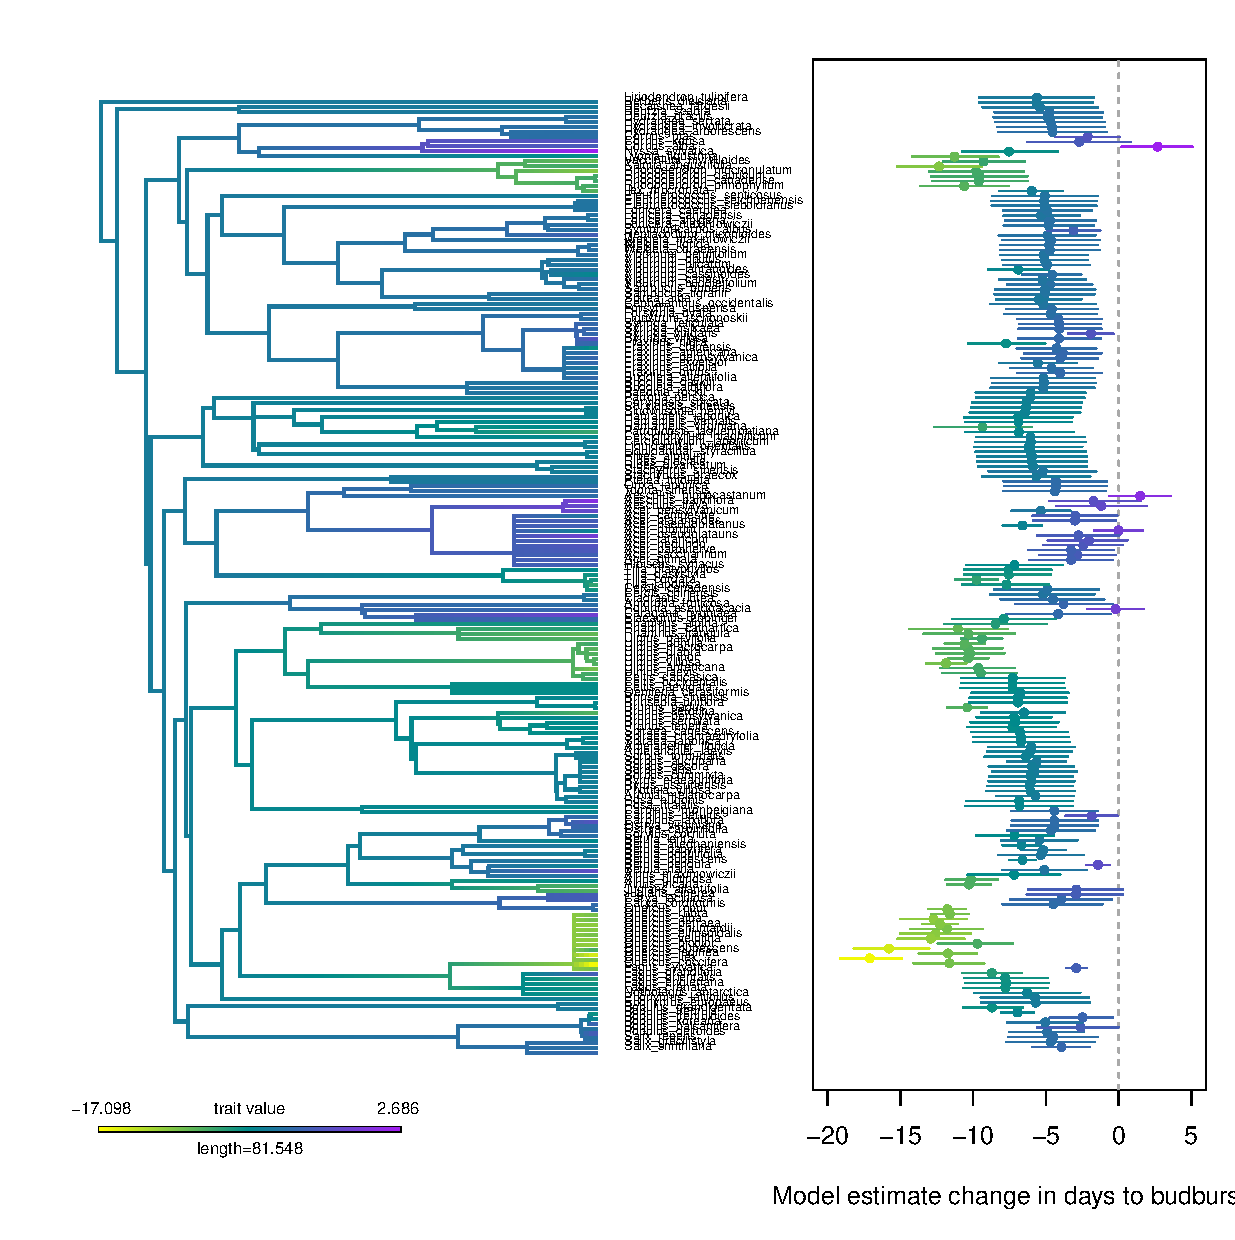
\includegraphics[width=14cm]{..//..//analyses/phylogeny/figures/muplot_phylo_force.pdf}
  \caption{Cue sensitivity estimation by hierarchical phylogenetic model showing slopes for forcing, for 194 angiosperm species.}
  \label{fig:muplot_force}
  \end{center}
\end{figure}

\begin{figure} [H]
  \begin{center}
  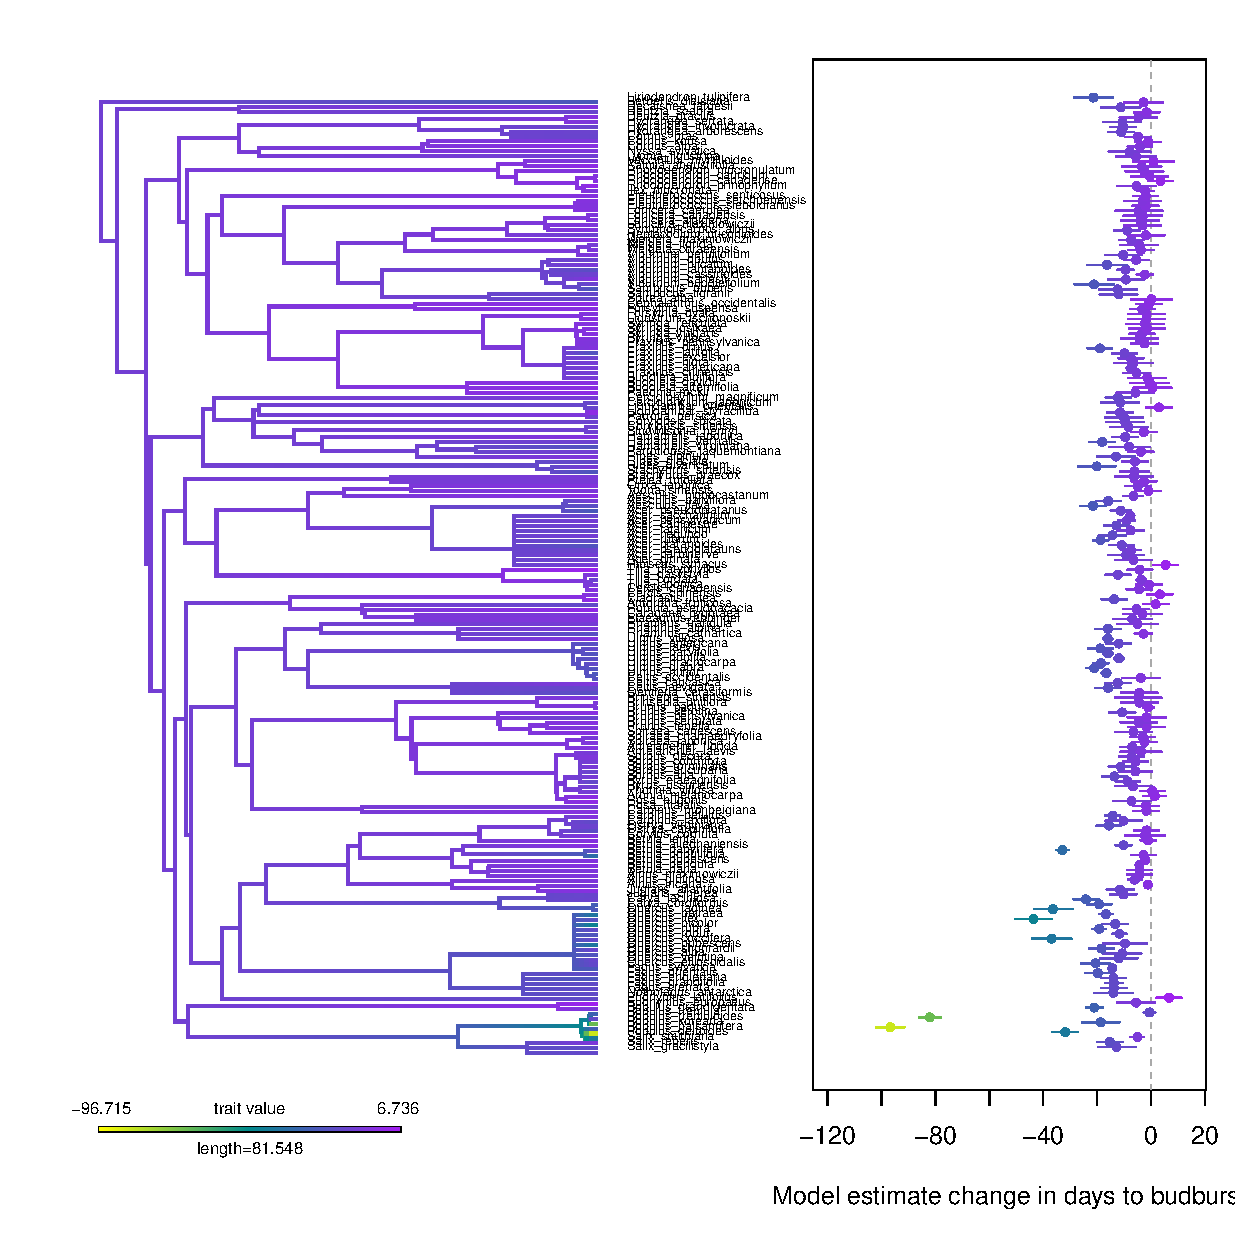
\includegraphics[width=14cm]{..//..//analyses/phylogeny/figures/muplot_phylo_chill.pdf}
  \caption{Cue sensitivity estimation by hierarchical phylogenetic model showing slopes for chilling, for 194 angiosperm species.}
  \label{fig:muplot_chill}
  \end{center}
\end{figure}

\begin{figure} [H]
  \begin{center}
  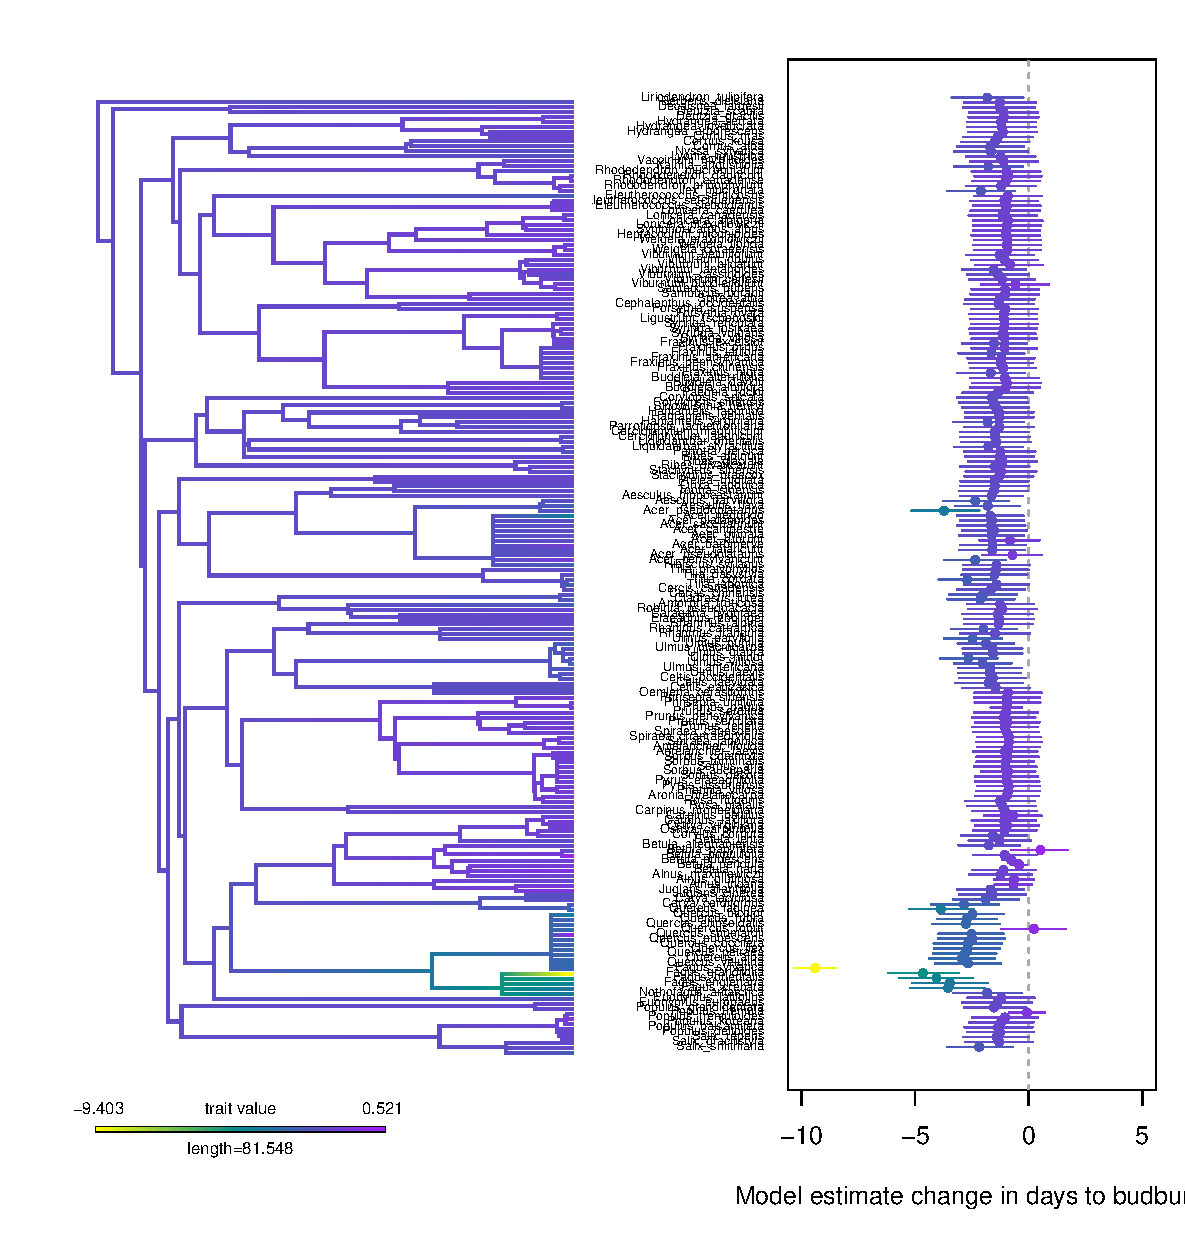
\includegraphics[width=14cm]{..//..//analyses/phylogeny/figures/muplot_phylo_photo.pdf}
  \caption{Cue sensitivity estimation by hierarchical phylogenetic model showing slopes for photoperiod, for 194 angiosperm species.}
  \label{fig:muplot_photo}
  \end{center}
\end{figure}


\begin{figure} [H]
  \begin{center}
  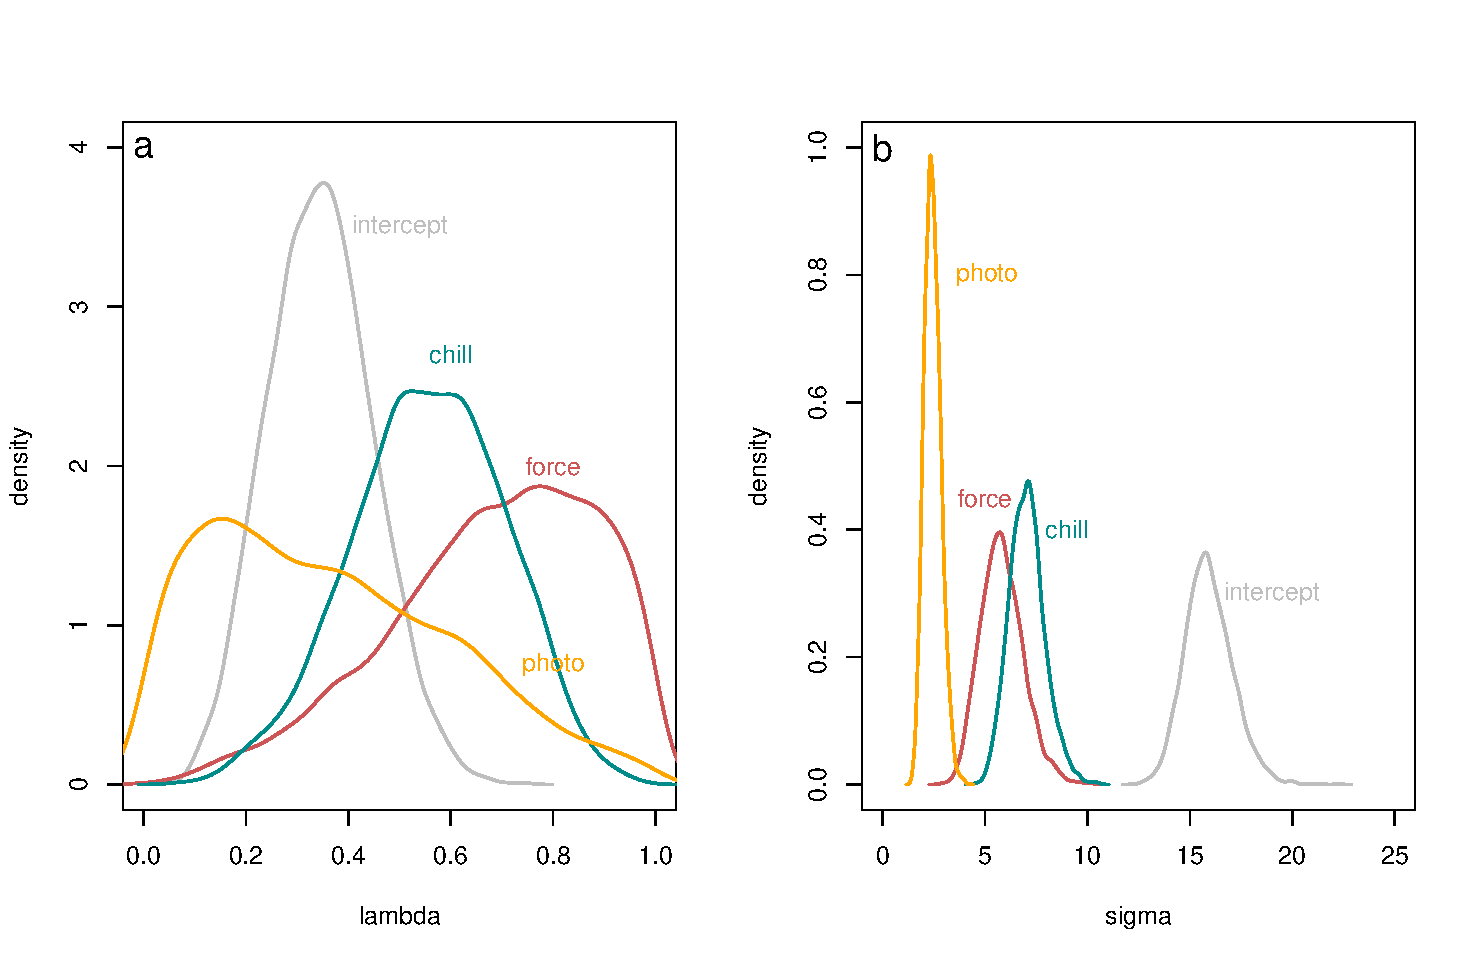
\includegraphics[width=14cm]{..//..//analyses/phylogeny/figures/lambdas_sigmas_density_noout.pdf}
  \caption{Posterior distribution of phylogenetic signal measured by lambda for each cue included as a predictor in the model for angiosperms: forcing (red), chilling (blue),  photoperiod (orange) and for the model intercept (grey).}
  \label{fig:phylosig_angio}
  \end{center}
\end{figure}

\begin{figure} [H]
  \begin{center}
  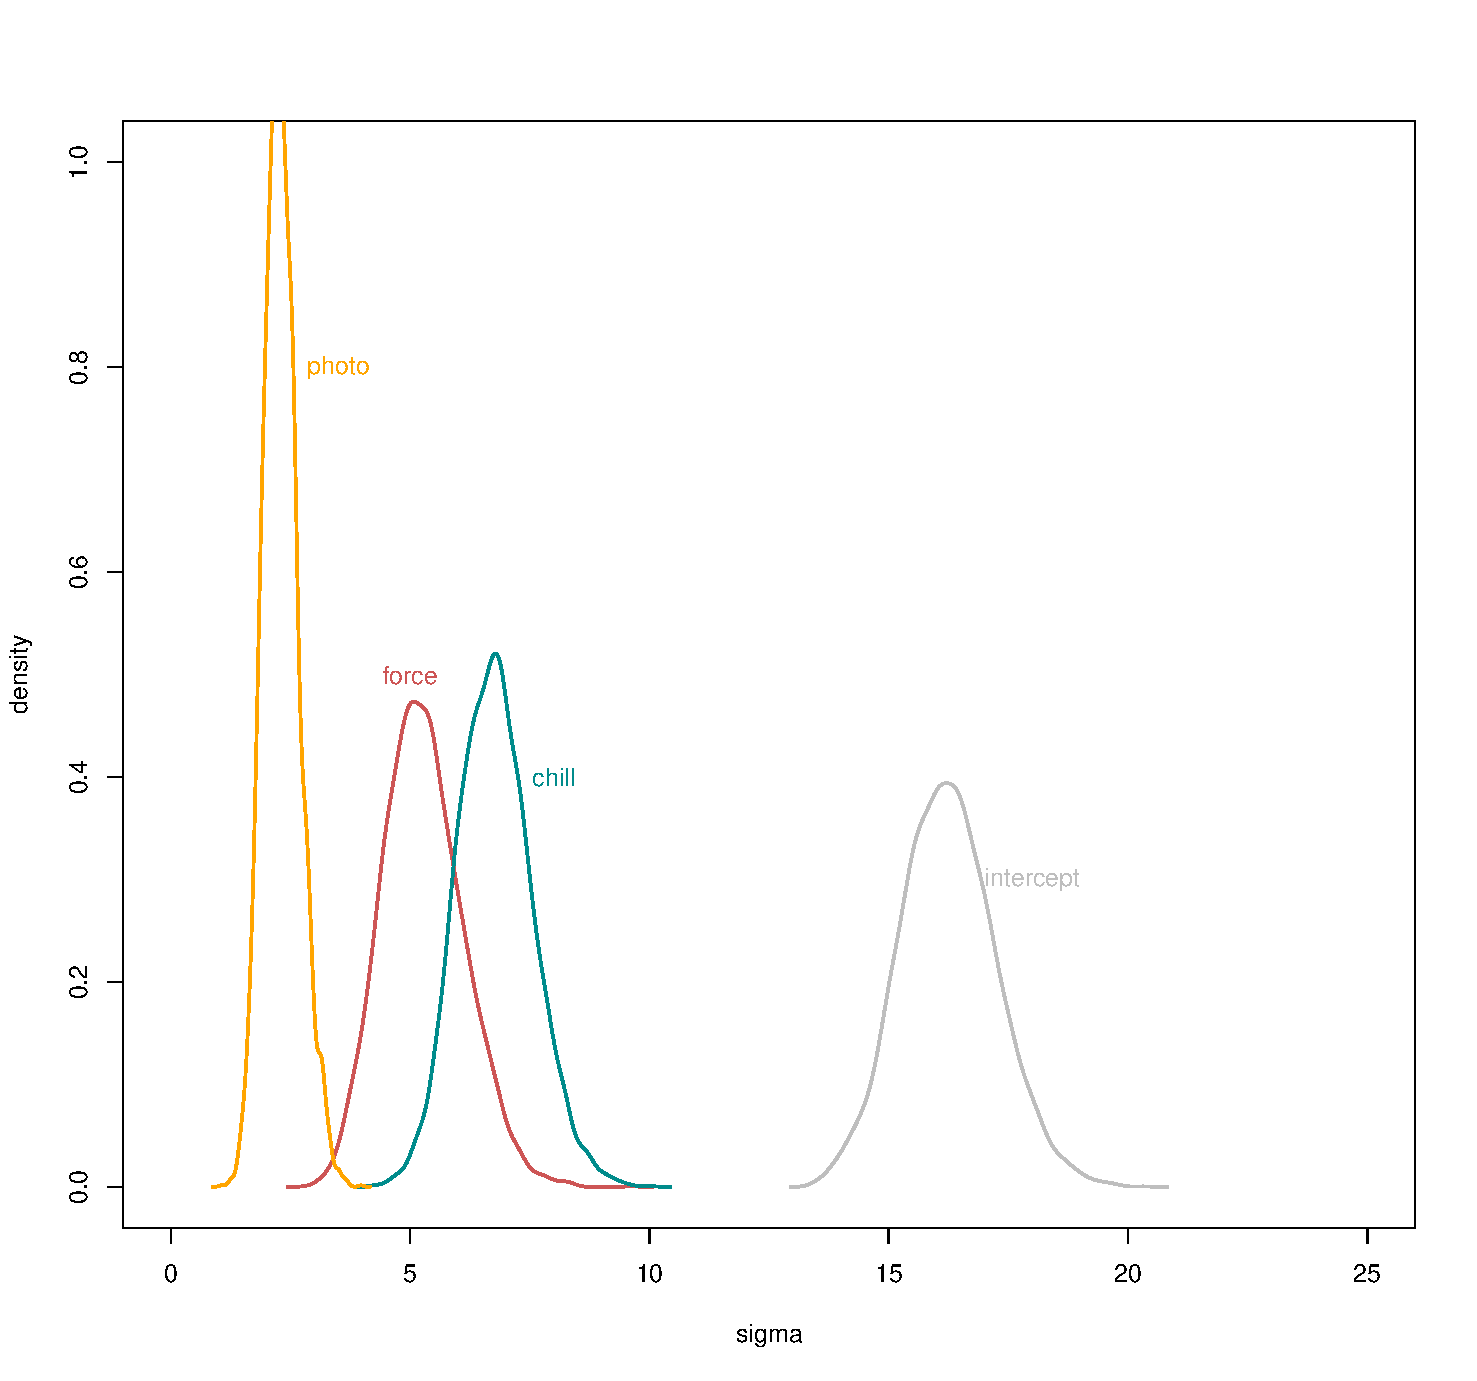
\includegraphics[width=14cm]{..//..//analyses/phylogeny/figures/sigmas_density_lambda0.pdf}
  \caption{Posterior distribution of sigma for each cue included as a predictor in the model for angiosperms: forcing (red), chilling (blue),  photoperiod (orange) and for the model intercept (grey).}
  \label{fig:sigmas}
  \end{center}
\end{figure}


\begin{figure} [H]
  \begin{center}
  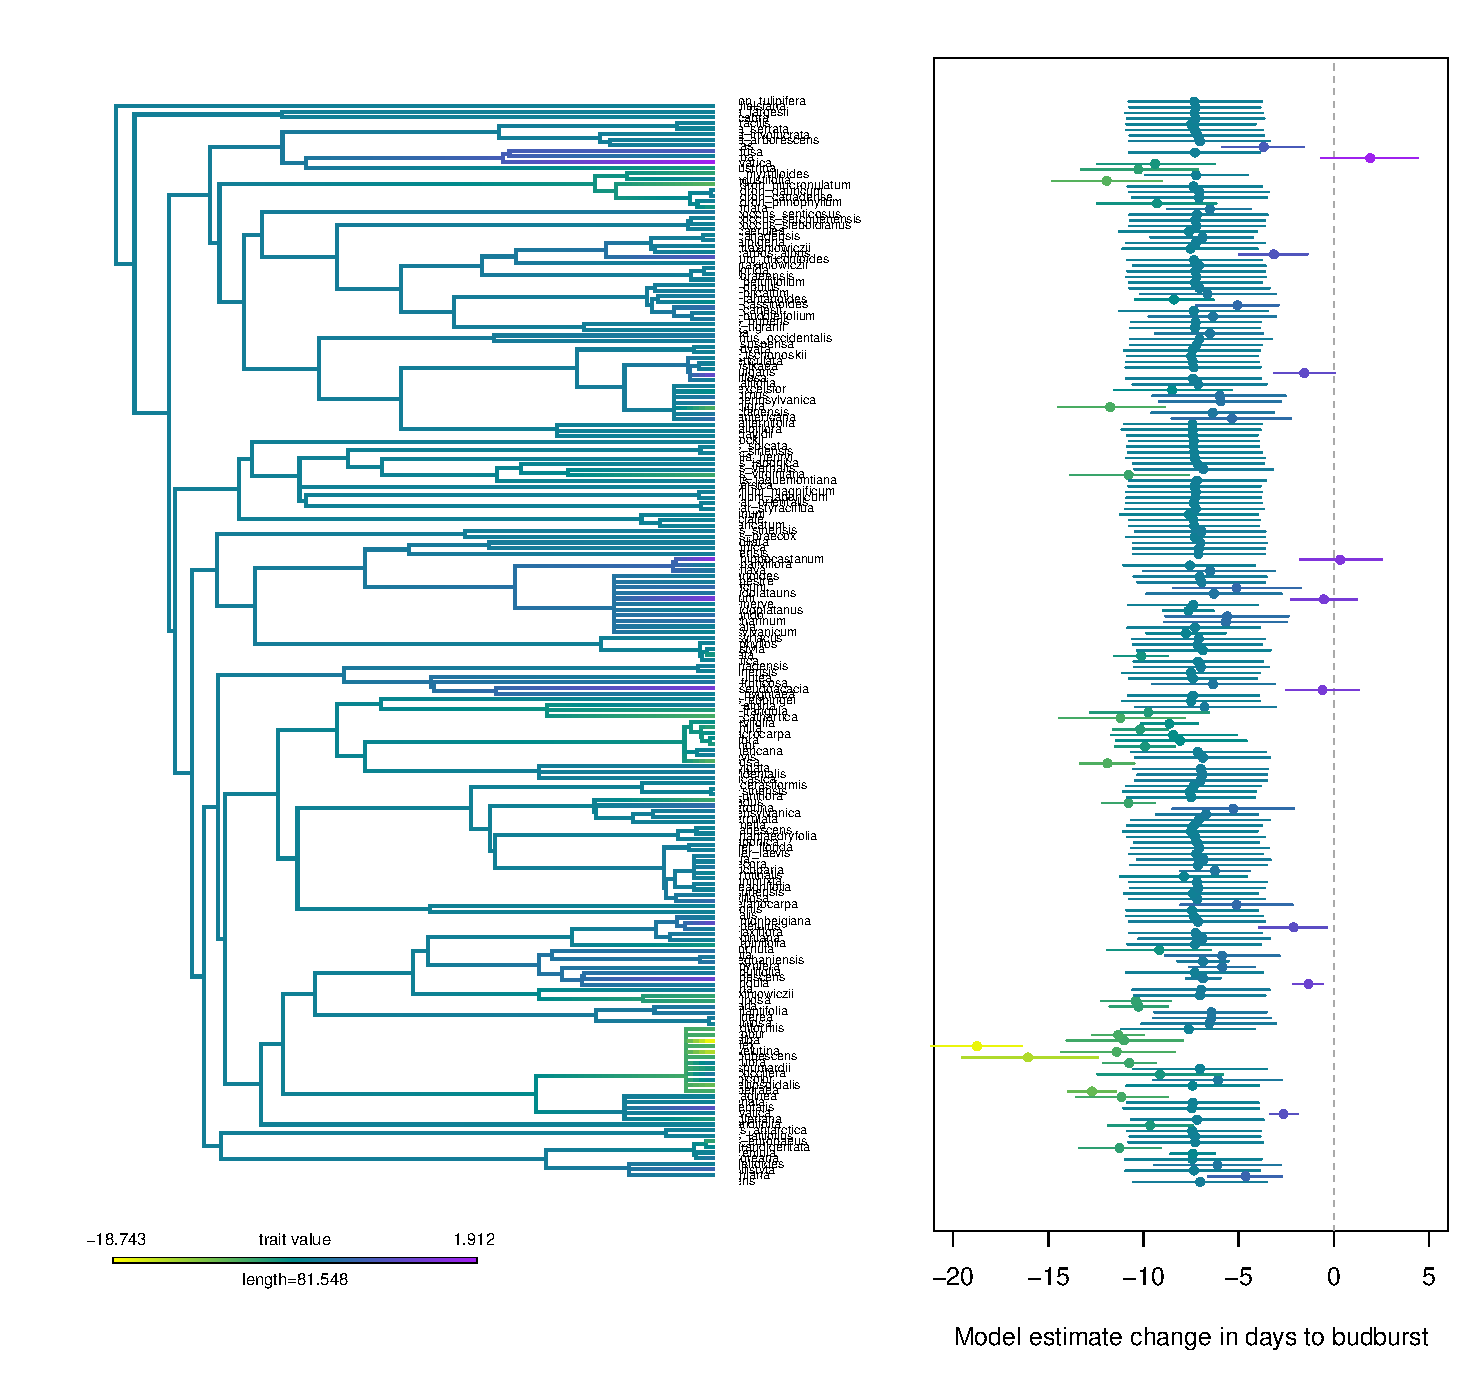
\includegraphics[width=14cm]{..//..//analyses/phylogeny/figures/muplot_phylo_force_lambda0.pdf}
  \caption{Cue sensitivity estimation by hierarchical phylogenetic model showing slopes for forcing making lambda \= 0, for 194 angiosperm species.}
  \label{fig:muplot_force_lambda0}
  \end{center}
\end{figure}

\begin{figure} [H]
  \begin{center}
  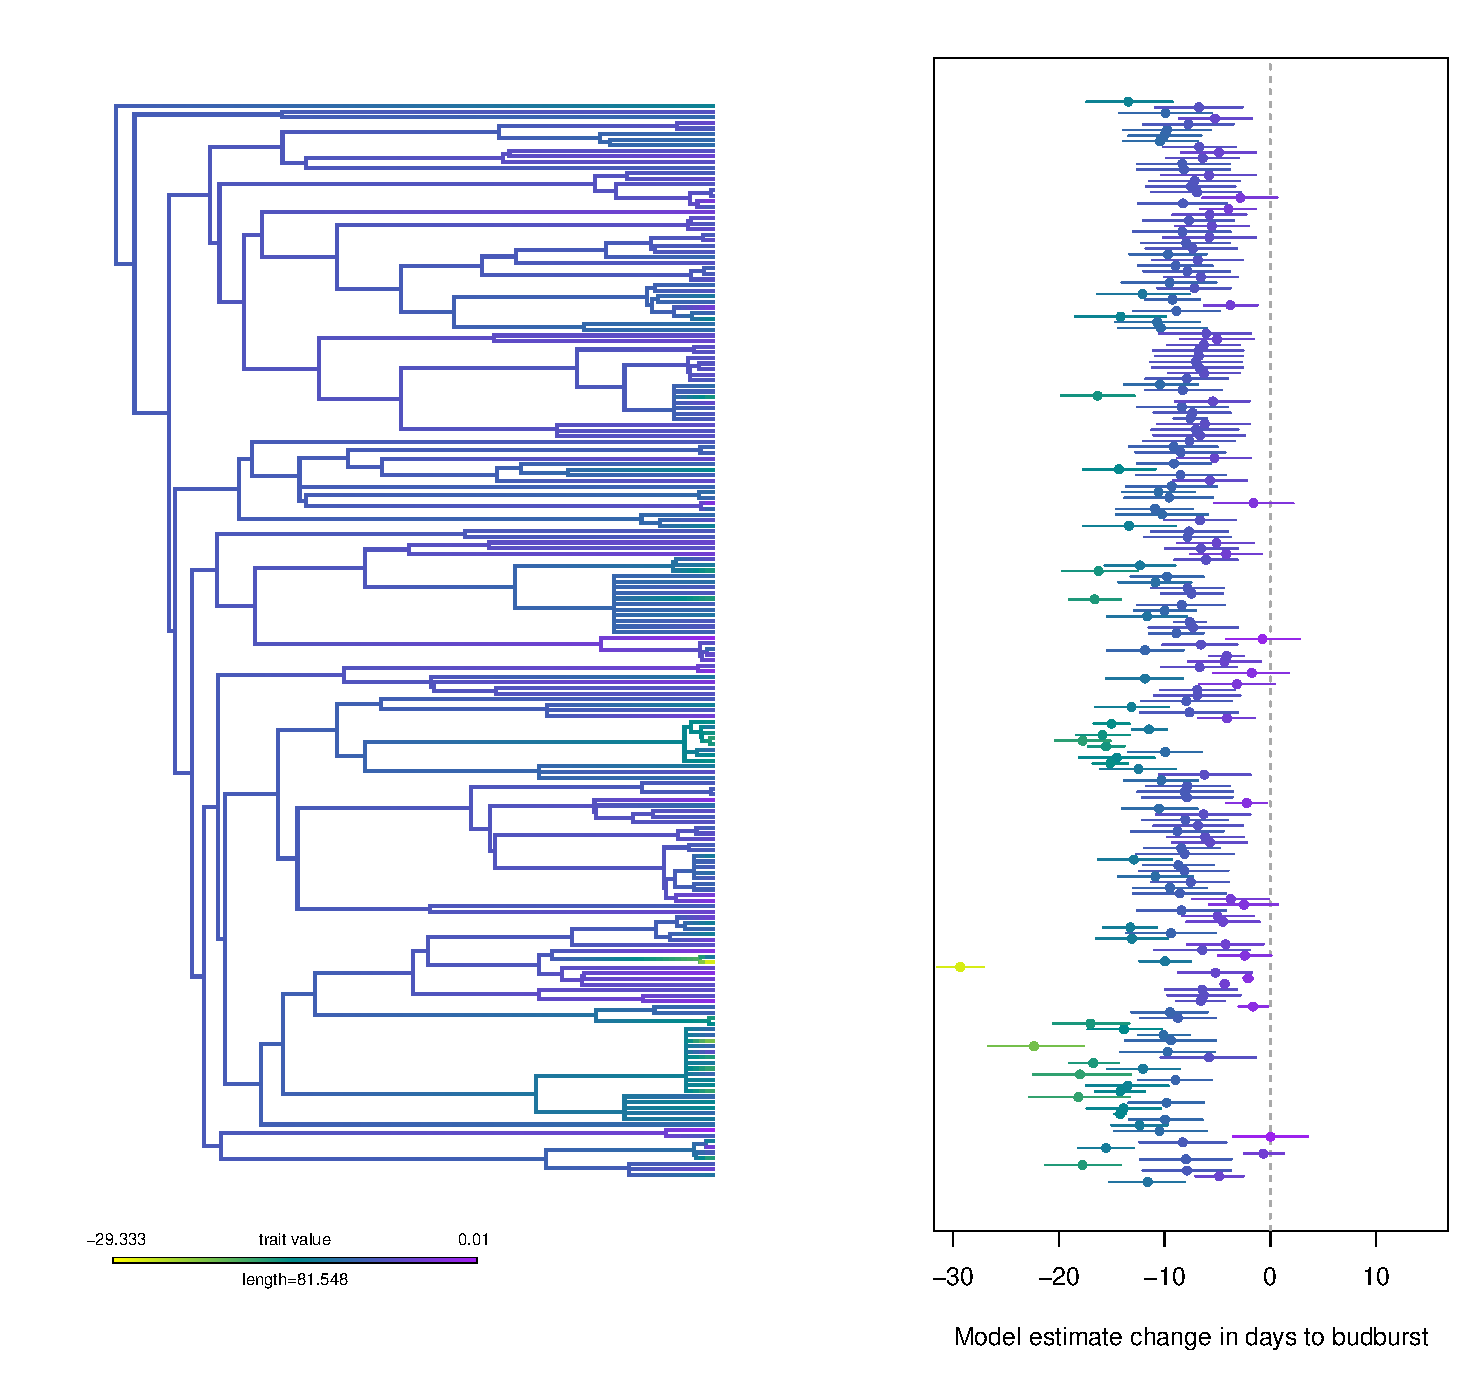
\includegraphics[width=14cm]{..//..//analyses/phylogeny/figures/muplot_phylo_chilll_lambda0.pdf}
  \caption{Cue sensitivity estimation by hierarchical phylogenetic model showing slopes for chilling making lambda \= 0, for 194 angiosperm species.}
  \label{fig:muplot_chill_lambda0}
  \end{center}
\end{figure}

\begin{figure} [H]
  \begin{center}
  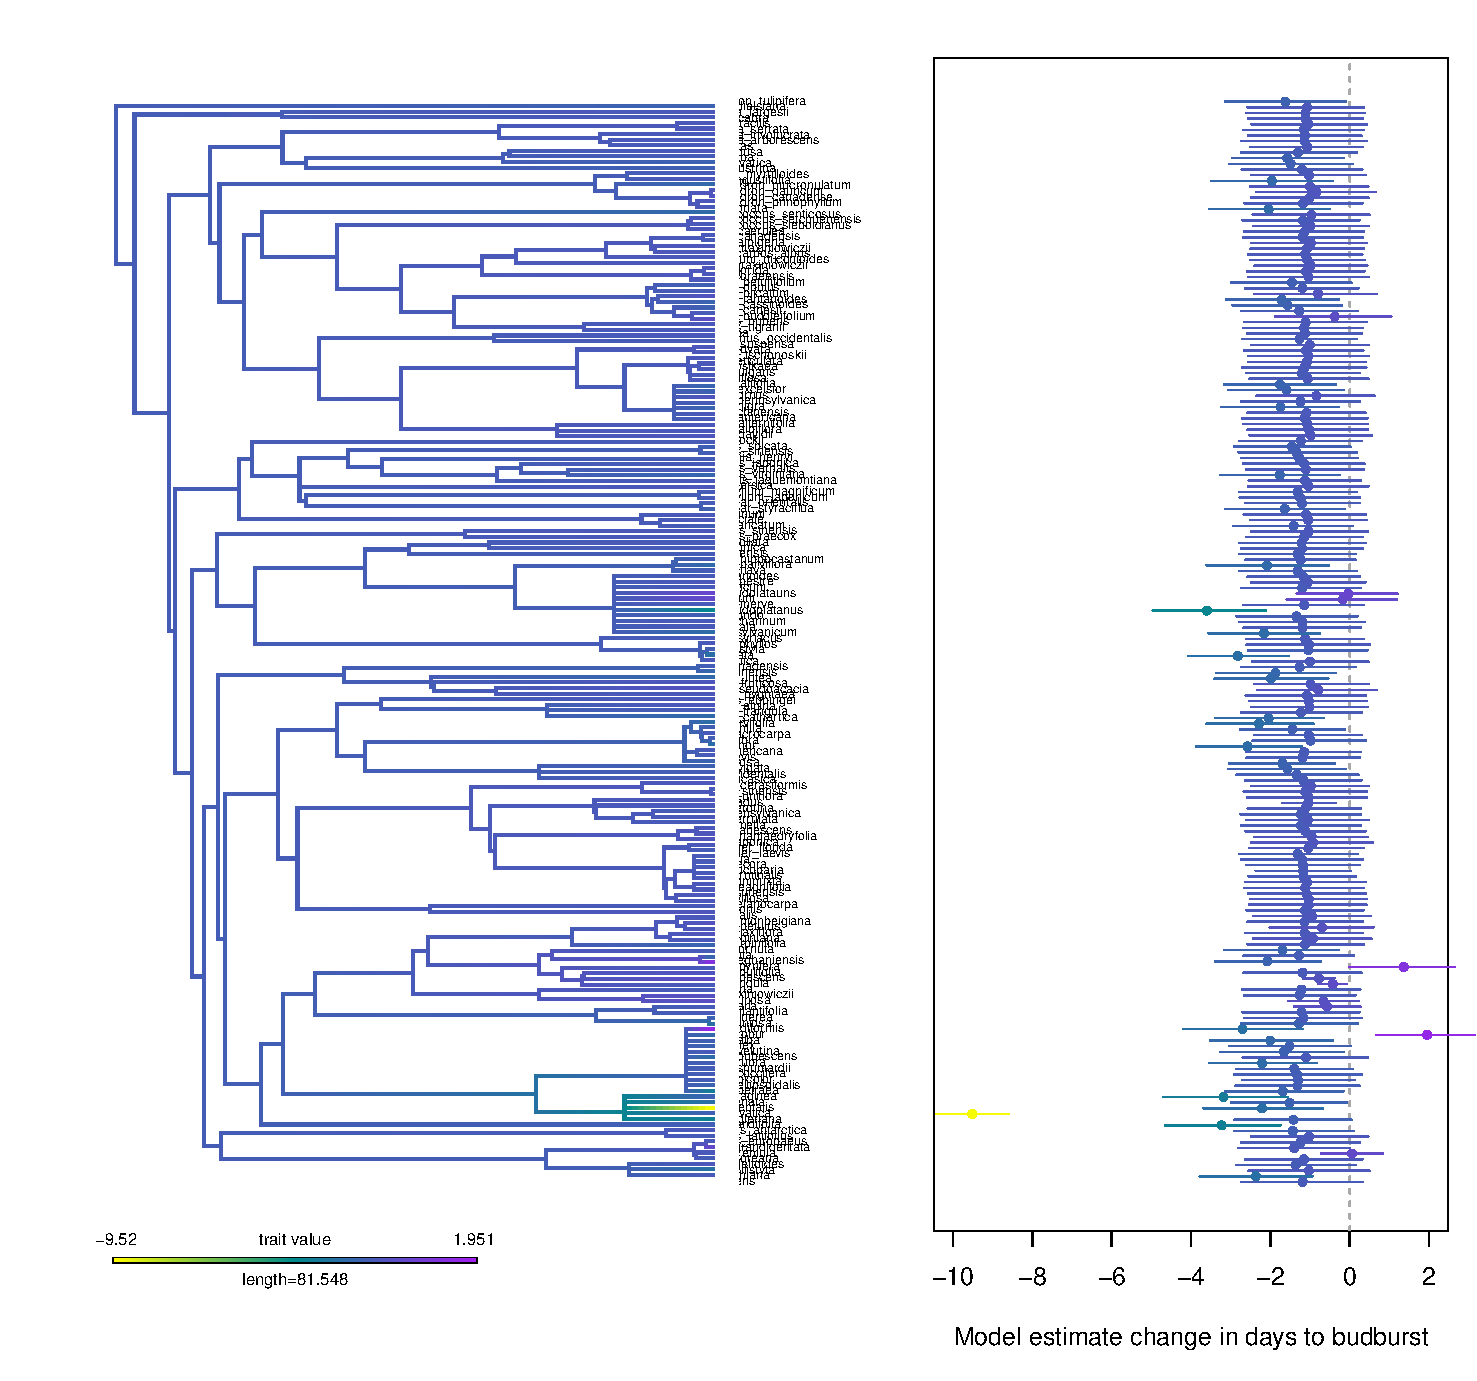
\includegraphics[width=14cm]{..//..//analyses/phylogeny/figures/muplot_phylo_photo_lambda0.pdf}
  \caption{Cue sensitivity estimation by hierarchical phylogenetic model showing slopes for photoperiod making lambda \= 0, for 194 angiosperm species.}
  \label{fig:muplot_photo_lambda0}
  \end{center}
\end{figure}


\begin{comment}
\begin{table}[H]
  \begin{center}

\caption{R2 estimates for models fitted to two subsets of data.}
\begin{tabular}{@{}llcccc@{}}
\toprule
Model                        & nsps & R2    & Est.Error & Q2.5  & Q97.5 \\ \midrule
mod.sps.intercept            & 52   & 0.369 & 0.012     & 0.346 & 0.392 \\
mod.sps.phylo.intercept      & 52   & 0.370 & 0.012     & 0.345 & 0.393 \\
mod.sps.interc.slope         & 52   & 0.478 & 0.011     & 0.456 & 0.498 \\
mod.sps.interc.slope.phy.int & 52   & 0.478 & 0.011     & 0.455 & 0.499 \\
mod.sps.intercept            & 117  & 0.369 & 0.012     & 0.344 & 0.393 \\
mod.sps.phylo.intercept      & 117  & 0.369 & 0.012     & 0.345 & 0.392 \\
mod.sps.interc.slope         & 117  & 0.486 & 0.011     & 0.465 & 0.506 \\
mod.sps.interc.slope.phy.int & 117  & 0.487 & 0.011     & 0.465 & 0.507 \\
mod.sps.intercept            & 215  & 0.582 & 0.007     & 0.566 & 0.596 \\
mod.sps.phylo.intercept      & 215  & 0.582 & 0.007     & 0.567 & 0.596 \\
mod.sps.interc.slope         & 215  & 0.659 & 0.006     & 0.646 & 0.670 \\
mod.sps.interc.slope.phy.int & 215  & 0.658 & 0.006     & 0.646 & 0.671 \\ \bottomrule
\end{tabular}
 \label{table:R2table}
  \end{center}

 \end{table}


\begin{table}[H]
  \begin{center}

\caption{Leave One Out analyses for models fitted to two subsets of data.}
\begin{tabular}{@{}llrrcc@{}}
\toprule
Model                        & nsps & elpd\_diff & se\_diff & elpd\_loo  & se\_elpd\_loo \\ \midrule
mod.sps.interc.slope         & 52   & 0.000      & 0.000    & -10944.890 & 75.627        \\
mod.sps.interc.slope.phy.int & 52   & -0.090     & 0.366    & -10944.980 & 75.572        \\
mod.sps.phylo.intercept      & 52   & -217.806   & 24.087   & -11162.696 & 74.662        \\
mod.sps.intercept            & 52   & -218.150   & 24.041   & -11163.040 & 74.719        \\
mod.sps.interc.slope.phy.int & 117  & 0.000      & 0.000    & -10951.579 & 75.858        \\
mod.sps.interc.slope         & 117  & -0.543     & 0.591    & -10952.122 & 75.803        \\
mod.sps.phylo.intercept      & 117  & -242.375   & 25.727   & -11193.955 & 75.031        \\
mod.sps.intercept            & 117  & -242.582   & 25.691   & -11194.161 & 75.097        \\
mod.sps.interc.slope         & 215  & 0.000      & 0.000    & -14195.898 & 89.929        \\
mod.sps.interc.slope.phy.int & 215  & -1.945     & 2.411    & -14197.843 & 90.075        \\
mod.sps.phylo.intercept      & 215  & -302.843   & 27.217   & -14498.741 & 89.759        \\
mod.sps.intercept            & 215  & -305.035   & 27.306   & -14500.933 & 89.765        \\ \bottomrule
\end{tabular}
 \label{table:lootable}
   \end{center}
\end{table}

\begin{table}[H]
\begin{center}
\caption{Comparison between phylogenetic signal from PGLS and BRMS.}
\begin{tabular}{@{}llllllll@{}}
\toprule
subset     & cue      & $\lambda$      & Lower95CI   & Upper95CI   & $H^2$          & Lower95CI   & Upper95CI   \\ \midrule
52-complex & forcing  & 0.171446841 & NA          & 0.650638627 & 0.330834872 & 0.008358609 & 0.751811447 \\
           & chilling & 1.00E-06    & NA          & 0.396954468 & 0.194753034 & 0.000682814 & 0.610910681 \\
           & photo    & 0.655354248 & 0.186405507 & 0.897899618 & 0.662218791 & 0.208150902 & 0.920502832 \\ \bottomrule
\end{tabular}
 \label{table:phylosigtable}
\end{center}
\end{table}





\clearpage
\begin{figure} [H]
  \begin{center}
  \includegraphics[width=14cm]{..//..//analyses/phylogeny/figures/correlations_sensitiv_52complex.png}
  \caption{Scatterplots showing correlations between the sensitivities of the species complexes in OSPREE to chilling and photoperiod (A), chilling and forcing (B), and forcing and photoperiod (C). Sensitivities are positively correlated among chilling and photoperiod and chilling and forcing, but negatively correlated between forcing and photoperiod.}
  \label{fig:sensicorrs}
  \end{center}
\end{figure}

\clearpage
\begin{figure} [H]
  \begin{center}
  \includegraphics[width=14cm]{..//..//analyses/phylogeny/figures/Correlations_sensitivities.png}
  \caption{Scatterplots showing correlations between the sensitivities of the species in OSPREE to chilling and photoperiod (A), chilling and forcing (B), and forcing and photoperiod (C). Sensitivities are  correlated overall, but more so between chilling and photoperiod.}
  \label{fig:sensicorrs52comp}
  \end{center}
\end{figure}

\begin{figure} [H]
  \begin{center}
  \includegraphics[width=14cm]{..//..//analyses/phylogeny/figures/cues_sensit_correlations_231spp.png}
  \caption{Scatterplots showing correlations between the sensitivities of the species in OSPREE (subset with all 231 species for which there is data) to chilling and photoperiod (A), chilling and forcing (B), and forcing and photoperiod (C). Sensitivities are positively correlated among chilling and photoperiod and chilling and forcing, but negatively correlated between forcing and photoperiod.}
  \label{fig:sensicorrs231}
  \end{center}
\end{figure}


\clearpage
\begin{figure} [H]
  \begin{center}
  \includegraphics[width=14cm]{..//..//analyses/phylogeny/figures/Sensitivities_phylosig.png}
  \caption{Phylogenetic signal results for the sensitivities of each species complex (species grouped by genera) to the forcing (A), chilling (B) and photoperiod (C) cues.}
  \label{fig:phylosig_complex}
\end{center}
\end{figure}

\begin{figure} [H]
  \begin{center}
  \includegraphics[width=14cm]{..//..//analyses/phylogeny/figures/Sensitivities_phylosig_spslev.png}
  \caption{Phylogenetic signal results for the sensitivities of each species (ungrouped) to the forcing (A), chilling (B) and photoperiod (C) cues.}
  \label{fig:phylosig_spp}
  \end{center}
  \end{figure}

\begin{figure} [H]
  \begin{center}
  \includegraphics[width=14cm]{..//..//analyses/phylogeny/figures/Sensitivities_phylosig_spslev_angiosperms.png}
  \caption{Phylogenetic signal results for the sensitivities of each species (excluding gymnosperms) to the forcing (A), chilling (B) and photoperiod (C) cues.}
  \label{fig:phylosig_angiosperm}
  \end{center}
\end{figure}

\begin{figure} [H]
  \begin{center}
  \includegraphics[width=14cm]{..//..//analyses/phylogeny/figures/Sensitivities_phylosig_spslev231.png}
  \caption{Phylogenetic signal results for the sensitivities of each species (231 species included) to the forcing (A), chilling (B) and photoperiod (C) cues.}
  \label{fig:phylosig_231spp}
  \end{center}
\end{figure}

\begin{figure} [H]
  \begin{center}
  \includegraphics[width=14cm]{..//..//analyses/phylogeny/figures/Sensitivities_phylosig_spslev215angio.png}
  \caption{Phylogenetic signal results for the sensitivities of each species (215 angiosperm only species included) to the forcing (A), chilling (B) and photoperiod (C) cues.}
  \label{fig:phylosig_215spp}
  \end{center}
\end{figure}



%%%%%%%%%%%%%%%%%%%%%%%%%%%%%%%
% Stuff from old version of the ms.
%%%%%%%%%%%%%%%%%%%%%%%%%%%%%%%
\section*{Stuff from old version (to be deleted at some point)} 

\subsection*{Hierarchical models to estimate species-level cue sensitivity}
\begin{enumerate}
\item Our approach used Bayesian hierarchical models to estimate the number of days until budburst as a function of forcing, chilling and photoperiod. We used different specifications of partial pooling to determine in which approach the sensitivies to the cues most accurately predict budburst. We used 5 model specifications: 
\begin{enumerate}
\item species as a grouping factor on the intercept (Eq. \ref{eq:1})
\item species as grouping factor on the intercept and slopes too (Eq. \ref{eq:2})
\item phylogeny as a grouping factor on the intercept and species as grouping factor on both  intercept and slopes (Eq. \ref{eq:3})
\item phylogeny as a grouping factor on the intercept and species as grouping factor on both  intercept and slopes (Eq. \ref{eq:3})

\end{enumerate}

\item In all specifications, the Bayesian hierarchical models were fit using the brms package \citep{brms}, in R \citep{R}, version 3.5.1, and followed the notations: 


\begin{equation}
\label{eq:1} 
Budbreak = \alpha_{species} + \beta_{1}forcing 
+ \beta_{2}chilling + \beta_{3}photo + \varepsilon
\end{equation}


\begin{equation} 
\label{eq:2} 
Budbreak = \alpha_{spp} + \beta_{1,spp}forcing
+ \beta_{2,spp}chilling + \beta_{3,spp}photo + \varepsilon\end{equation}

\begin{equation} 
\label{eq:3} 
Budbreak = \alpha_{phylo,spp} + \beta_{1,spp}forcing
+ \beta_{2,spp}chilling + \beta_{3,spp}photo + \varepsilon
\end{equation}

\begin{equation} 
\label{eq:4} 
Budbreak = \alpha_{phylo,species} + \beta_{1}forcing
+ \beta_{2}chilling + \beta_{3}photo + \varepsilon
\end{equation}

% I'm ignoring the model below for now as it runs very slow, and it does not seem like we are using it
%\begin{equation} 
%\label{eq:5} 
%Budbreak = \alpha_{phylo,spp} + \beta_{1, phylo, spp}forcing +\\
% \beta_{2, phylo, spp}chilling + \\
% \beta_{3, phylo, spp}photo + \varepsilon
%\end{equation}


\item We assessed model performance according to $\hat{R}$ values (that should be close to one to ensure convergence). As for metrics of model accuracy we computed $R^{2}$, and the expected log predictive density (ELPD) that results from \emph{Leave-one-out} cross-validation, in addition to inspection of posterior predictive checks.

\item To test the ability of phylogeny to improve models/predictions of budburst we compared metrics of model accuracy between models that include phylogeny and models that do not.

\end{enumerate}


\begin{enumerate}
% Explain how the model is fit, and how the $H^{2}$ metric is analogous to lambda in PGLS.
\item To determine phylogenetic signal in the responses to each of the environmental cues--i.e. forcing, chilling, photoperiod--we run a second batch of models in brms, that use the slopes of the models specified above as a response variable, following the notation:



\begin{equation}
\label{eq:5} 
\beta_{1}forcing = \alpha_{phylo} + \varepsilon_{phylo} + \varepsilon_{non-phylo}
\end{equation}

\begin{equation}
\label{eq:6} 
\beta_{2}chilling = \alpha_{phylo} + \varepsilon_{phylo} + \varepsilon_{non-phylo}
\end{equation}

\begin{equation}
\label{eq:7} 
\beta_{3}photo = \alpha_{phylo} + \varepsilon_{phylo} + \varepsilon_{non-phylo}
\end{equation}

\item Once this set of models is computed, calculating phylogenetic signal ($H^{2}$) is straightforward:

\begin{equation}
\label{eq:8} 
\quad   H^{2} = \frac{\varepsilon_{phylo}}{\varepsilon_{phylo} + \varepsilon_{non-phylo}}
\end{equation}

\item $H^{2}$ is equivalent to Pagel's \cite{pagel1999inferring} $\lambda$ parameter \citep{housworth2004phylogenetic}, constrained to range from 0 to 1, with values of 0 indicating absence of phylogenetic relatedness, and values of 1 indicating \emph{Brownian Motion} evolution (BM). This is, for $\lambda = 0$ phylogenetically close species are not more similar than phylogenetically distant species and, for $\lambda = 1$, phylogenetically close species resemble each other according to a BM model, where phenotypic variance accummulates proportional to time.

\item In other words, the $\lambda$ parameter can be defined as a scalar that multiplies the diagonal of the phylogenetic Variance-Covariance metric and that is estimated through \emph{Maximum Likelihood} in traditional comparative approaches \citep{freckleton2002phylogenetic}. Our approach, in contrast computes the ratio between amount of variance attributable to the phylogeny ($\varepsilon_{phylo}$) and the total amount of variance \ref{eq:8}.
\todo{Results from our approach and PGLS differ in the 215spp dataset - to discuss} 

\item We compare the results from our $H^{2}$ metric against the results for $\lambda$ computed through Phylogenetic Generalized Least Squares \citep{freckleton2002phylogenetic}. 
%\item An advantage of estimating phylogenetic signal through a Bayesian approach such as ours is that it yields a posterior distribution of $H^{2}$.

\end{enumerate}



%% from previous version of the intro outline
\item Few examples in the literature have tested for phylogenetic signal of phenological responses using growth chamber data (e.g. \cite{joly2019importance}, and yet such a source of data could have advantages such as:
\begin{enumerate}
\item it makes possible to examine responses to more than one cue and thus not restrict analyses to responses to forcing.
\item it is possible to compare responses to cues (are some more conserved than others?) 
\item they may allow testing whether phylogeny can improve models of phenology as a response to a cue
\end{enumerate}

\item Shifting the focus to phylogenetic conservatism of the responses to cues may provide additional insights:
\begin{enumerate}
\item by allowing comparison across cues, which cues are more conserved? which selective processes have been stronger? 
\item Do we need to care about phylogenetic constraints when we forecast phenology? 
\item Understand what dimensions of the environment may be more limiting or may be less subject to further adaptation. 
\item Is the phylogenetic conservatism of phenology affected by geography and/or taxonomy? (e.g. North America vs. Europe; Gymnosperms vs. Angiosperms) 
\end{enumerate}

\subsection*{Provenance-climate Data}
\begin{enumerate}
\item Should we test/analyze provenace or climate-effects? 
\todo{I belive this can be done (roughly) through the NAm vs. Eur comparison?} 
\end{enumerate}

\section*{Next steps and directions (based on Lizzie's suggestions)}
\begin{enumerate}
\item Compute phylogenetic signal on the outcome of the cues -- that is, we could calculate budburst day given our model (maybe a model without phylogeny?) under perhaps two scenarios:
     
\begin{enumerate}
\item High chill, long-ish photoperiod, and moderate forcing (regular scenario)

\item Low chill, shorter photoperiod, higher forcing (climate change scenario)

\item The trick will be first, which model to use to calculate these values and how to keep the paper then logically consistent.
\end{enumerate}
  
\end{enumerate}


\section*{Questions to be addressed}

Some questions we need to answer (suggestions by Lizzie and Nacho's addings):

\begin{enumerate}
\item How do we approach wanting to use species-level output from the models and wanting to fit phylogenetically-informed models? I think our current approach of using phylo-corrected and uncorrected models is fine, but we should discuss.
\item Do we want to compare North America and Europe somehow? sounds cool!
\item Do we want to add any traits or range stuff? - I don't think I'd go there unless there is a really pressing question or idea to address
\item Can people add refs? Especially recent refs and refs about leafout and budburst? We also should have some refs on WITHIN-species variation. This is a task that would be great if people could contribute.
\item Would it make sense to look at other response variables in OSPREE (other than budburst)?\\

And a very important question:\\

\item How do we want to pitch this paper? About phenology? About moving beyond phenotypes? About using experimental (lab) data? About climate change forecasts being affected by phylogenetic structuring?

\item If the latter, can we think of ways to show how accounting for phylogenetic structuring would affect (or best case scenario, improve) forecasts of phenology? Perhaps by focusing on well studied species (usual PEP75 suspects?)... 

\item Probably still early for this, but any ideas for target journals? JoE seems a natural outlet given where previous work has been published, but if the pitch is more into forecasts, could we aim higher?
\end{enumerate}

\end{comment}

\end{document}
